In this section we will discuss the results given by our Monte Carlo simulation of 2D Ising model. 
Sec. \ref{sec:2times2result} gives the results of $2 \times 2$ case for benchmark. 
In Sec. \ref{sec:detailresult} we discuss the change of energy and magnetization in the Monte Carlo process for $20\times20$ lattice 
and show their probability distributions. 
In Sec. \ref{sec:transitionresult} the phenomenon of phase transition in 2D Ising model is discussed for different lattice size. 

\subsection{Benchmark: $2 \times 2$ case}\label{sec:2times2result}
\begin{table}[tb]
	\centering
	\caption{Results for $2\times2$ case with temperature $T=1.0$. Analytical results are provided for benchmark. 
	Energy is in the unit of $J$. }
	\begin{tabular}{cccccc}
		\hline
		\hline
		Number of Monte Carlo cycles $MC$ & 10 & 100 & 1000 & 10000 & Analytical \\ 
		\hline
		Mean energy $\langle E \rangle$ & -7.2 & -7.92 & -7.986 & -7.988 & -7.98393\\ 
		Mean magnetization $\langle |M| \rangle$ & 3.75 & 3.975 & 3.9955 & 3.99625 & 3.99263\\ 
		Mean square of energy $\langle E^2 \rangle$ & 57.6  & 63.36 & 63.888 & 63.904 & 63.8714\\ 
		Mean square of magnetization $\langle M^2 \rangle$ & 14.7 & 15.87 & 15.977 & 15.9805 & 15.9732\\ 
		Heat capacity $C_V$ & 5.76 & 0.6336 & 0.111804 & 0.095856 & 0.128329\\ 
		Susceptibility $\chi$ & 0.6375 & 0.069375 & 0.0129798 & 0.0104859 & 0.0320873\\ 
		\hline
		\hline 
	\end{tabular} 
	\label{tab:2times2result}
\end{table}
Table \ref{tab:2times2result} gives the quantities we obtain from our Monte Carlo simulation of $2\times2$ lattice with temperature $T=1.0$. 
As the number of Monte Carlo cycles $MC$ increases, our results get closer to the analytical values. 
For $MC=1000$ our results are close enough to the analytical values for benchmark purpose. 
However, we can notice that both heat capacity $C_V$ and susceptibility $\chi$ do not agree well with the analytical results, 
and they have some fluctuations as $MC$ increases. 
The reason is that both $\langle E^2 \rangle$ and $\langle E \rangle^2$ are large but close to each other, 
so their difference, which determines $C_V$, will have a large numerical error. 
This is unavoidable when $C_V$ and $\chi$ are small. 

\subsection{Details in the Monte Carlo process}\label{sec:detailresult}
\begin{figure}[tb]
	\begin{subfigure}[tb]{0.5\textwidth}
		\centering
		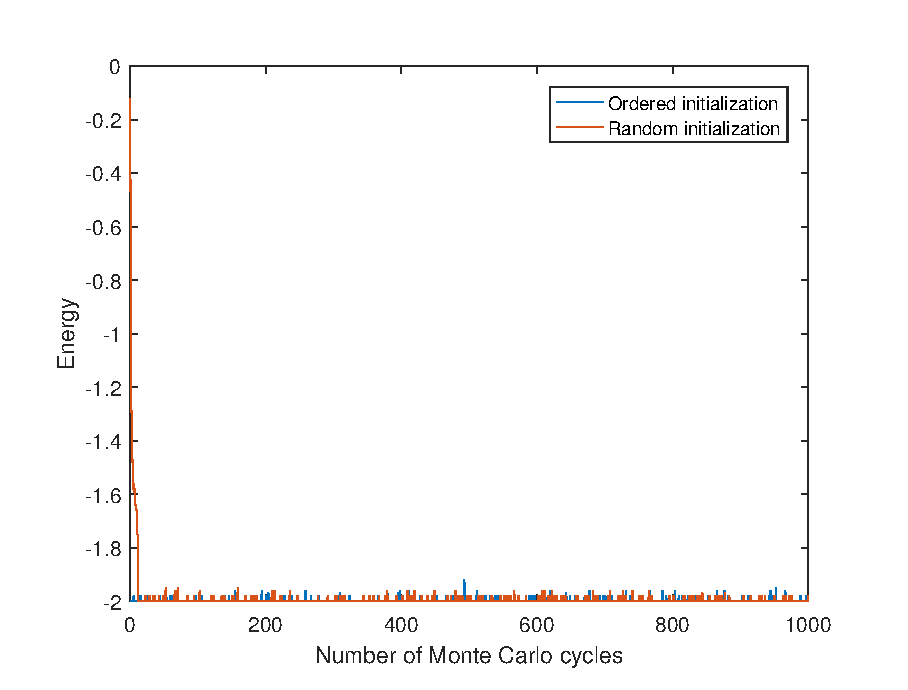
\includegraphics[width=0.7\textwidth]{Process_ene_lowT.eps}
		\caption{$T=1.0$}
	\end{subfigure}
	~
	\begin{subfigure}[tb]{0.5\textwidth}
		\centering
		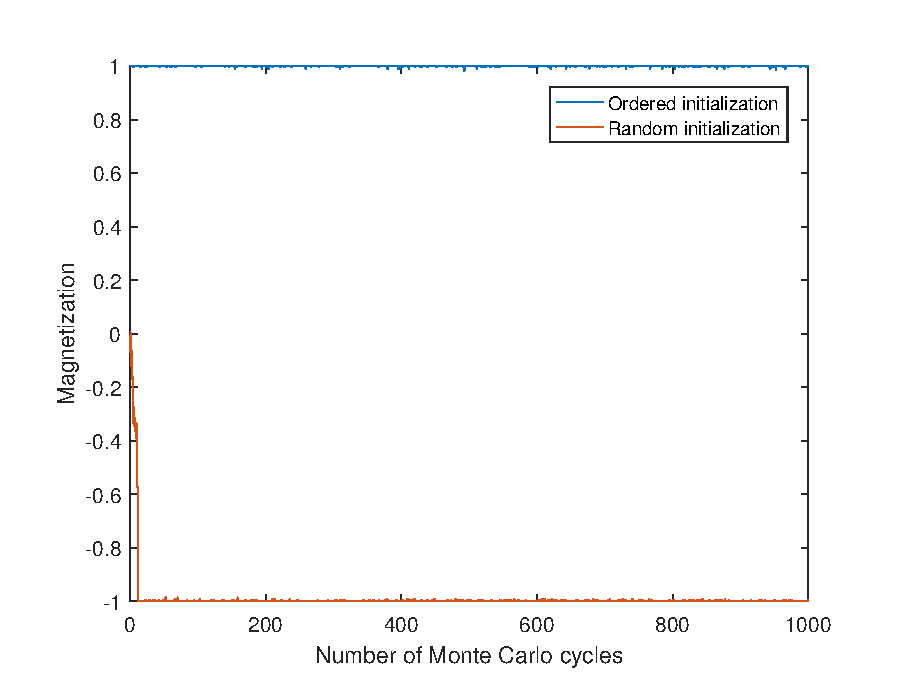
\includegraphics[width=0.7\textwidth]{Process_mag_lowT.eps}		
		\caption{$T=1.0$}
	\end{subfigure}
	~
	\begin{subfigure}[tb]{0.5\textwidth}
		\centering
		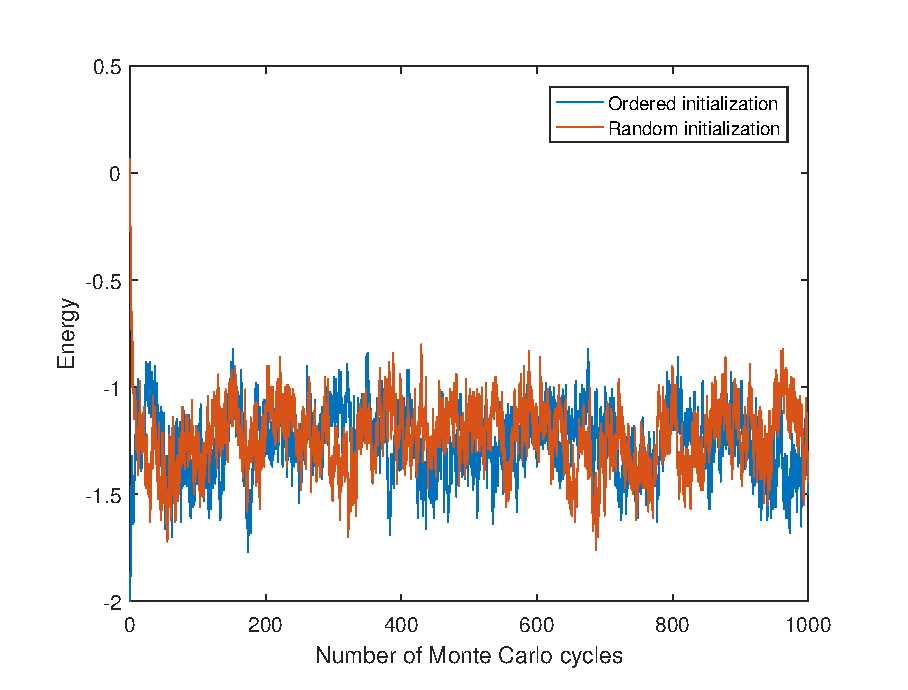
\includegraphics[width=0.7\textwidth]{Process_ene_highT.eps}		
		\caption{$T=2.4$}
	\end{subfigure}
	~
	\begin{subfigure}[tb]{0.5\textwidth}
		\centering
		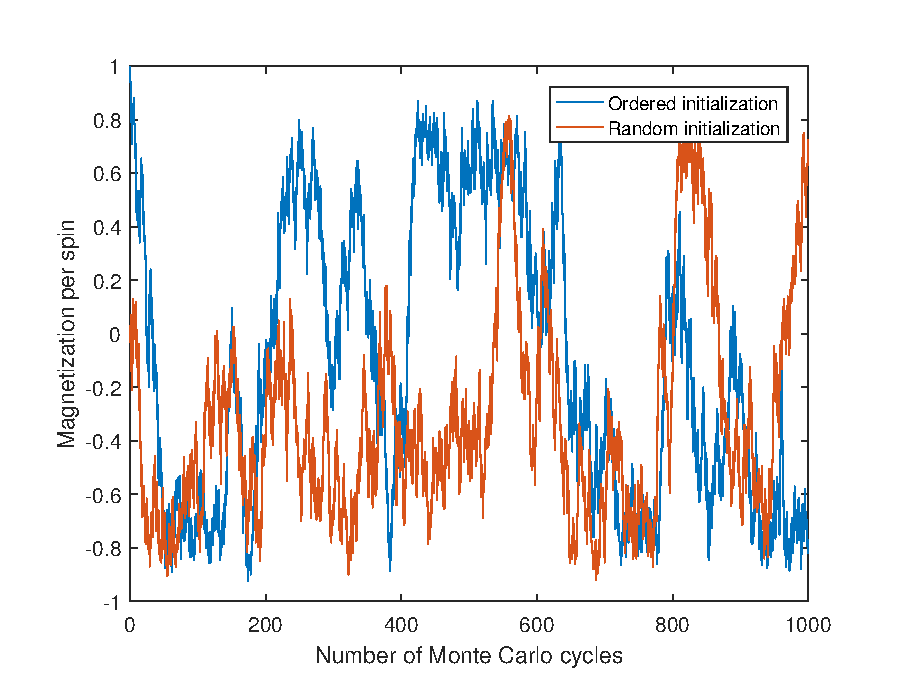
\includegraphics[width=0.7\textwidth]{Process_mag_highT.eps}		
		\caption{$T=2.4$}
	\end{subfigure}
	\caption{Energy and magnetization as a function of the number of Monte Carlo cycles. 
	Energy is in the unit of $J$. Temperature $T=1.0$ or $2.4$. }
	\label{fig:process}
\end{figure}
For our simulation, it is important to know when the properties of our system become equilibrated, 
which determines how many Monte Carlo cycles are necessary. 
Fig. \ref{fig:process} shows the change of energy and magnetization as a function of the number of Monte Carlo cycles $MC$ 
for $20 \times 20$ lattice with temperature $T=1.0$ and $T=2.4$. 
Blue lines are the results of ordered initialization (starting from all spins pointing up) 
and orange lines are the results of random initialization (starting from random spin orientation). 
From Fig. \ref{fig:process}, we can see that the energy of the system converges quite fast, 
and different initializations give the same results after some Monte Carlo cycles. 
For $T=1.0$, the system soon goes to an ordered phase with very small fluctuations. 
For $T=2.4$, higher temperature will raise the probability of the system being at excitation states. 
Thus, the energy has a larger fluctuation around its mean value, 
and the magnetization also oscillates dramatically 
because states with different magnetization can have the same energy (degeneracy). 
\par
\begin{figure}[tb]
	\begin{subfigure}[tb]{0.5\textwidth}
		\centering
		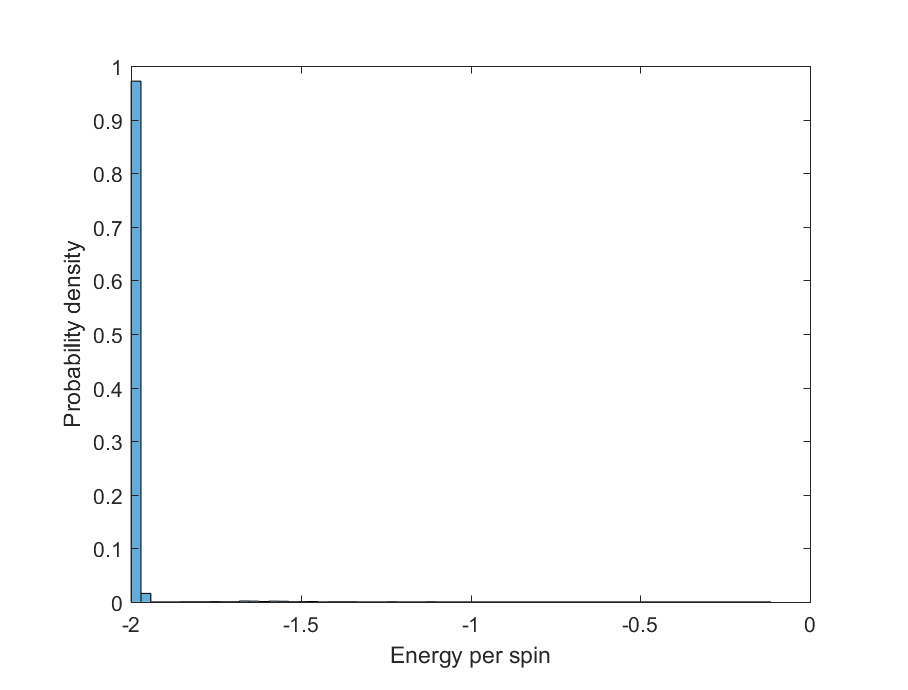
\includegraphics[width=0.7\textwidth]{Prob_ene_lowT.eps}
		\caption{$T=1.0$}
	\end{subfigure}
	~
	\begin{subfigure}[tb]{0.5\textwidth}
		\centering
		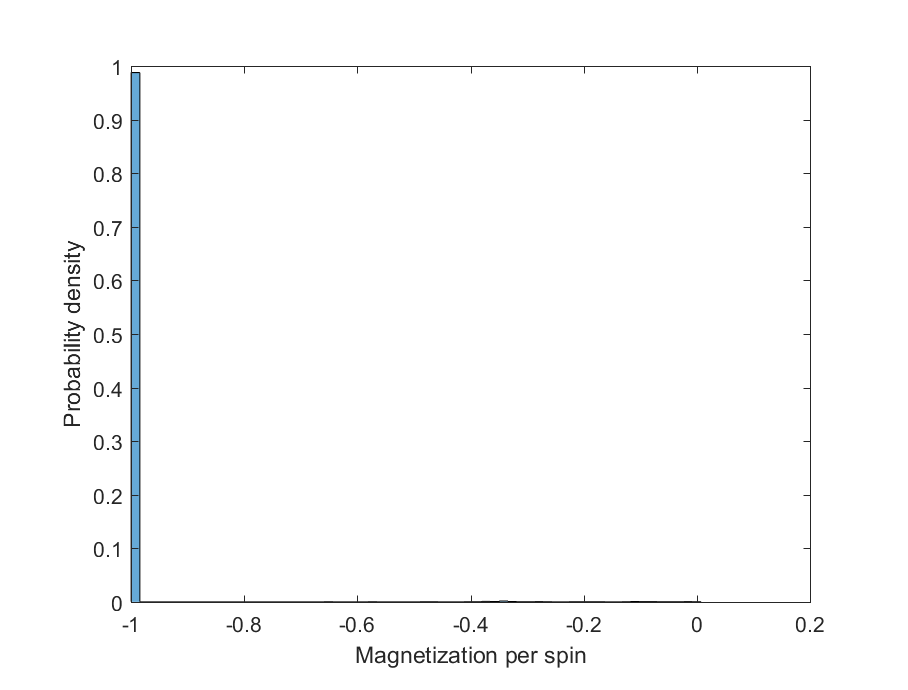
\includegraphics[width=0.7\textwidth]{Prob_mag_lowT.eps}		
		\caption{$T=1.0$}
	\end{subfigure}
	~
	\begin{subfigure}[tb]{0.5\textwidth}
		\centering
		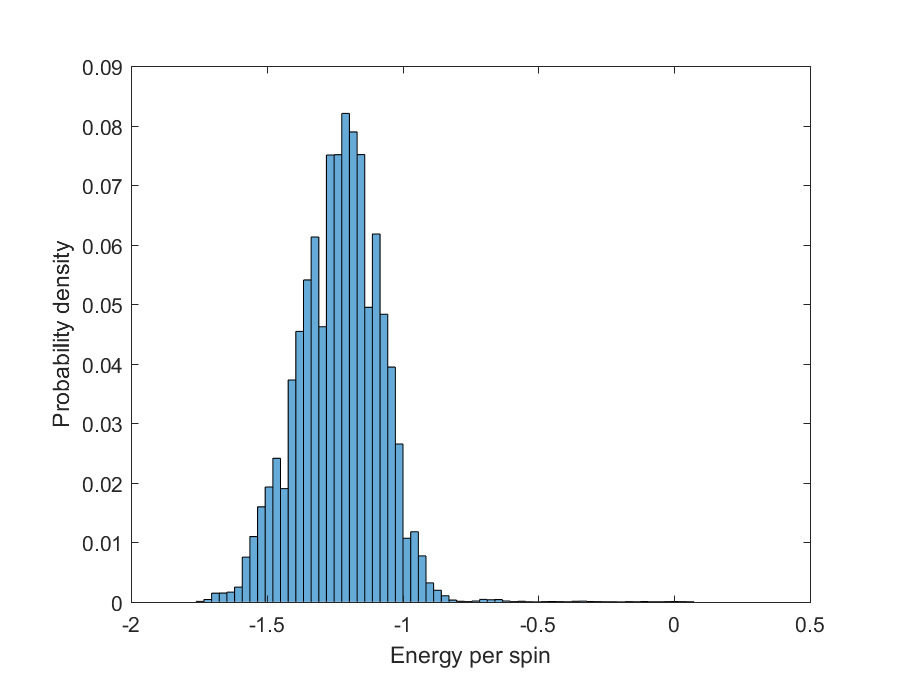
\includegraphics[width=0.7\textwidth]{Prob_ene_highT.eps}		
		\caption{$T=2.4$}
	\end{subfigure}
	~
	\begin{subfigure}[tb]{0.5\textwidth}
		\centering
		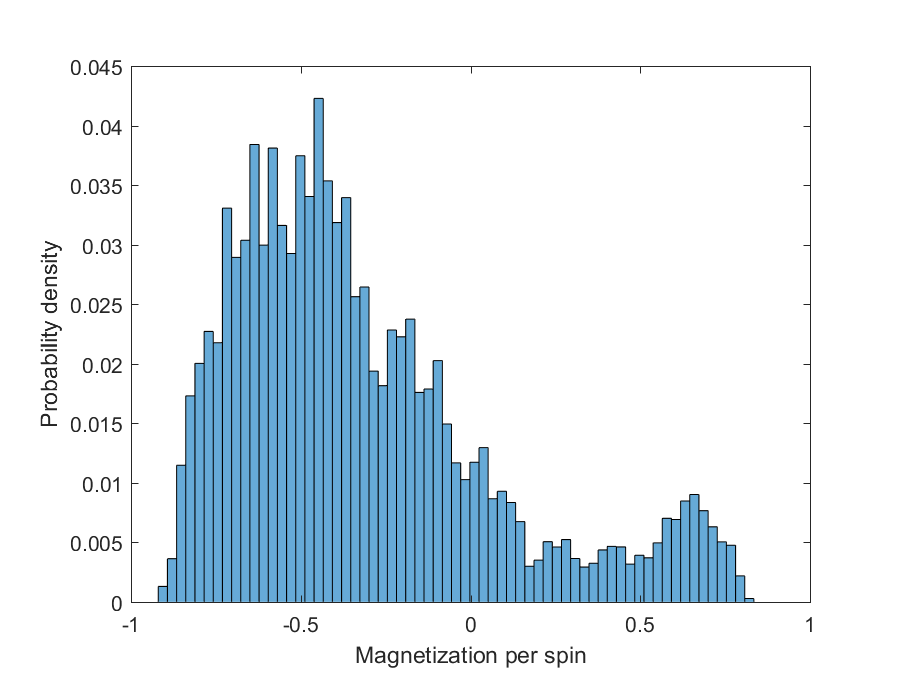
\includegraphics[width=0.7\textwidth]{Prob_mag_highT.eps}		
		\caption{$T=2.4$}
	\end{subfigure}
	\caption{Probability distribution of energy and magnetization per spin. 
		Energy is in the unit of $J$. Temperature $T=1.0$ or $2.4$. }
	\label{fig:prob}
\end{figure}
Fig. \ref{fig:prob} gives the distributions of energy and magnetization per spin in the Monte Carlo process with random initialization. 
For $T=1.0$, the system is almost always stays at an ordered phases, 
and thus we have a high peak of magnetization per spin at $M/L^2=1$, and a high peak of energy per spin at $E/L^2=-2$. 
For $T=2.4$, the distribution of energy centers at the most probable value, which is approximately the mean value; 
the distribution of magnetization is broader because of states with different magnetization but the same energy. 

\subsection{Phase transition}\label{sec:transitionresult}
\begin{figure}[tb]
	\begin{subfigure}[tb]{0.5\textwidth}
		\centering
		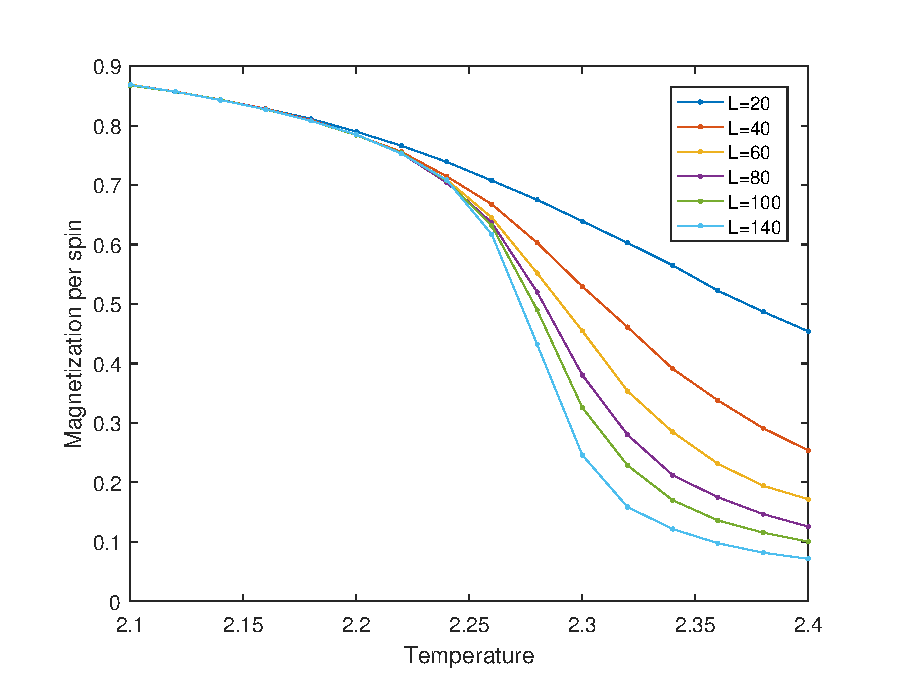
\includegraphics[width=0.7\textwidth]{Tran_mag.eps}
		\caption{}
	\end{subfigure}
	~
	\begin{subfigure}[tb]{0.5\textwidth}
		\centering
		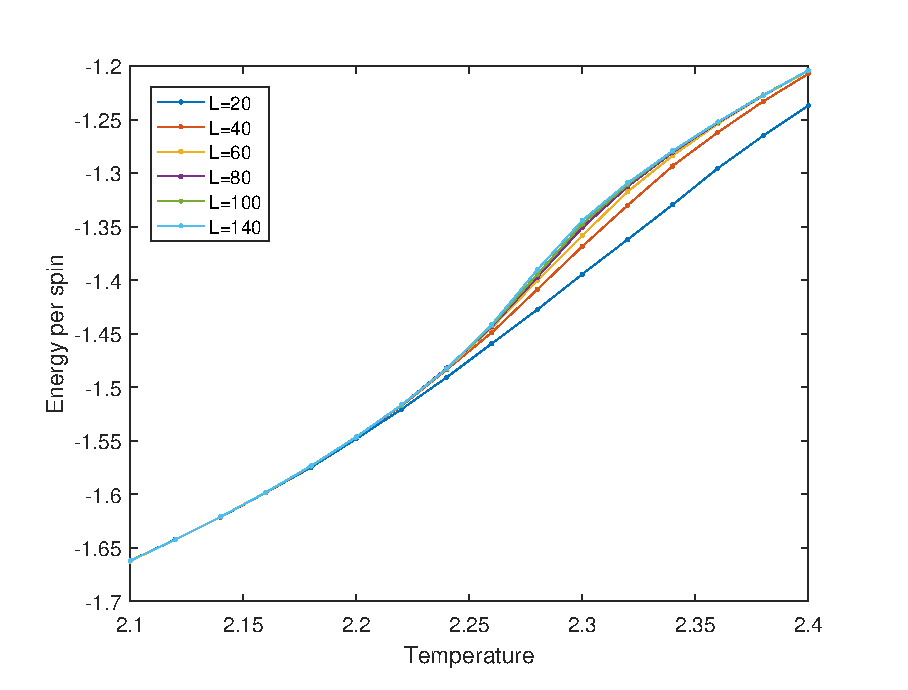
\includegraphics[width=0.7\textwidth]{Tran_ene.eps}		
		\caption{}
	\end{subfigure}
	~
	\begin{subfigure}[tb]{0.5\textwidth}
		\centering
		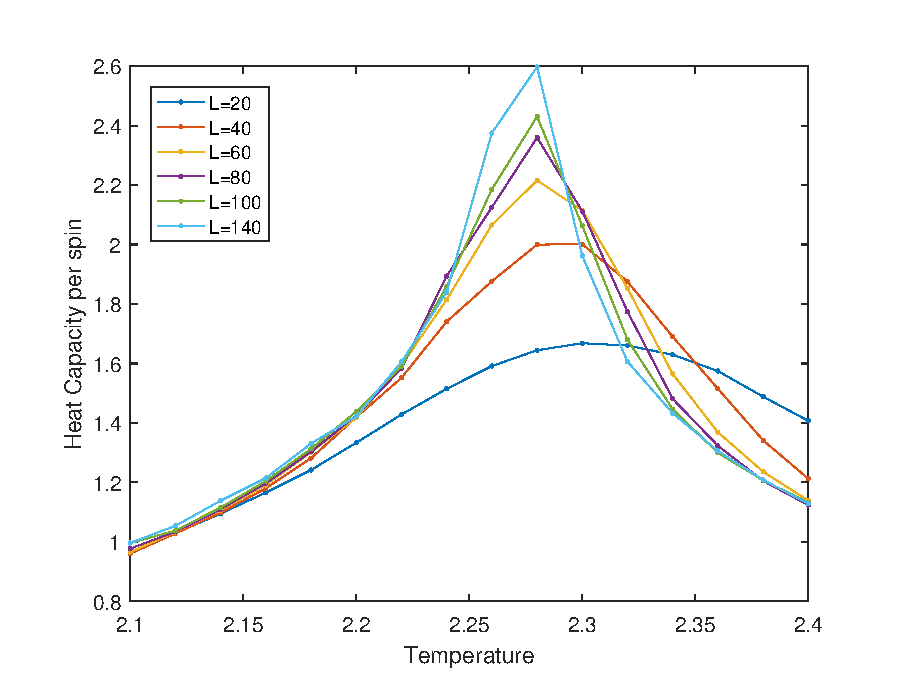
\includegraphics[width=0.7\textwidth]{Tran_Cv.eps}		
		\caption{}
	\end{subfigure}
	~
	\begin{subfigure}[tb]{0.5\textwidth}
		\centering
		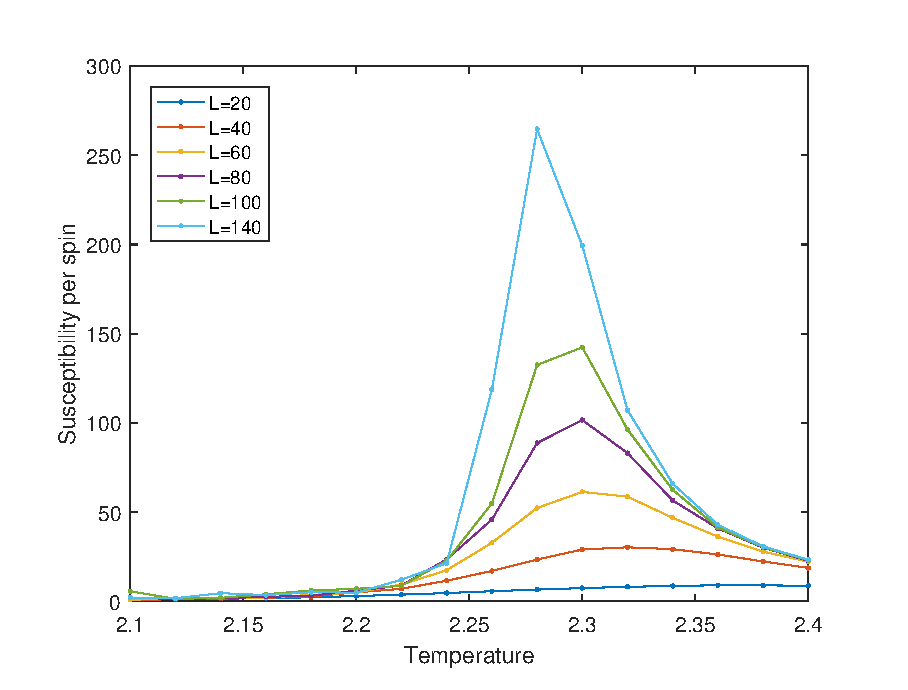
\includegraphics[width=0.7\textwidth]{Tran_sus.eps}		
		\caption{}
		\label{fig:transition_sus}
	\end{subfigure}
	\caption{Energy, magnetization, heat capacity and susceptibility per spin as a function of temperature
	with different lattice size $L=20,\,40,\,60,\,80,\,100,\,140$ in the temperature range $T\in[2.1,2.4]$. 
	Temperature step is 0.02. }
	\label{fig:transition}
\end{figure}
To investigate the phase transition in Ising model, we perform calculations with different lattice size 
$L=20,\,40,\,60,\,80,\,100,\,140$ in the temperature range $T\in[2.1,2.4]$. 
The temperature step is 0.02. 
Fig. \ref{fig:transition} gives the energy, magnetization, heat capacity and susceptibility per spin as a function of temperature. 
It can be seen that around $T=2.28$ the magnetization drops fast as $T$ increases, 
indicating that the system undergoes a transition from an ordered phase to a disordered phase. 
This transition is not dramatic when $L$ is small (e.g. $L=20$ and $40$), which results from the finite size of the system. 
The energy of the system, however, changes smoothly when the phase transition occurs, 
which is a characteristic of a second-order transition. 
Both heat capacity and susceptibility have a high peak around the transition temperature, 
which agrees with the divergence of these two quantities shown in the analytical solution. 
\par
By Eq. \ref{eq:tc} we can estimate $T_C$ for an infinitely large system from the results with finite $L$. 
It is quite difficult to determine the critical temperature from Fig. \ref{fig:transition} 
because our resolution is not small enough and the peaks of $C_V$ and $\chi$ do not coincide. 
From the peaks of $\chi$ (Fig. \ref{fig:transition_sus}) we estimate that $T_C(L=60)=2.3$ and $T_C(L=140)=2.28$. 
By Eq. \ref{eq:tc} and $\nu=1$ we obtain 
\begin{equation}
\left\{
\begin{array}{c}
a=2.1\,,  \\
T_C(L=\infty)=2.265\,.  \\
\end{array}
\right.
\end{equation}
Our estimation is not far from the analytical result 2.269. 